\section{Shape Detection}
\label{sec:shape_detection}

\subsection{Basics}

\textbf{Question 1:} Remind the principle of pseudo-inverse approach.

\TODO{}

The pseudo-inverse approach can be applied to find the best fit models to data. This is works well for linear models, such as 
\begin{equation}
    \Vec{y} = a \vec{x} + b 
\end{equation}
where $\vec{x} = (x_1, \dots, x_n)$ and $\vec{y} = (y_1, \dots, y_n)$ are our data points and $a$ and $b$ are the sought after parameters. The linear equation can be rewritten in matrix form for each data point as
\begin{equation}
    \underbrace{\begin{pmatrix}
        y_1 \\
        \vdots \\
        y_n
    \end{pmatrix}}_{Y}
    =
    \underbrace{\begin{pmatrix}
        x_1 & 1 \\
        \vdots & \vdots \\
        x_n & 1
    \end{pmatrix}}_{X}
    \underbrace{\begin{pmatrix}
        a \\ b
    \end{pmatrix}}_{P}
\end{equation}

The parameter vector is then found by inverting the equation to 
\begin{equation}
    P = X' Y 
\end{equation}

An alternative way to formulate the problem, which is handy when the equations aren't linear, is to write it out a linear relationship as follows:
\begin{equation}
    a\vec{x} + b\vec{y} + c = 0 \Leftrightarrow -\frac{a}{c} \vec{x} - \frac{b}{c} \vec{y} = 1 \equiv \alpha \vec{x} + \beta \vec{y} = 1 
\end{equation}

The matrix form is then expressed as
\begin{equation}
    \begin{pmatrix}
        x_1 & y_1 \\
        \vdots & \vdots \\
        x_n & y_n 
    \end{pmatrix} 
    \begin{pmatrix}
        \alpha \\
        \beta
    \end{pmatrix}
    = \mathbb{1} 
    \Leftrightarrow
    X P = \mathbb{1}
\end{equation}

The pseudo-inverse is then defined by multiplying by the transpose of $X$ on both sides, before inverting the equation:
\begin{equation}
    X^t X P = X^t \mathbb{1} \Rightarrow P = (X^t X)^{-1} X^t \mathbb{1}
\end{equation}
where the $pinv(X) = (X^t X)^{-1} X^t$ is the pseudo-inverse of $X$. With this formulation, more complex models that involve powers of $x$ and $y$ can be used to fit data. For example, an asteroid's trajectory is an ellipse, whose mathematical model is given by the expression
\begin{equation}
    a x^2 + 2 b x y + c y^2 + d x + e y = 1
    \label{eq:conicSectionRotated}
\end{equation}
Here we have both linear and quadratic terms, as well as cross-terms, which describe the overall shape and orientation of the ellipse. Each term is also not independent from each other, and we can reconstruct $d$ and $e$ from $a$, $b$ and $c$. Still, the pseudo-inverse can be constructed by arranging the terms in the matrix as follows:
\begin{equation}
    \begin{pmatrix}
        x_1^2  & 2 x_1 y_1 & y_1^2  & x_1    & y_1 \\
        \vdots & \vdots    & \vdots & \vdots & \vdots \\
        x_n^2  & 2 x_n y_n & y_n^2  & x_n    & y_n \\
    \end{pmatrix}
    \begin{pmatrix}
        a \\ b \\ c \\ d \\ e 
    \end{pmatrix} = \mathbb{1} 
\end{equation}

\textit{Now you observe a positions of an asteroid at different times, and the objective is to estimate its trajectory.}

\textbf{Question 2:} Complete the program \texttt{'AsteroidTry'} to estimate the asteroid trajectory. Detail the theoretical approach.

The well-known formula for an ellipse is given as
\begin{equation}
    \frac{(x - x_0)^2}{a^2} + \frac{(y - y_0)^2}{b^2} = 1
\end{equation}

This however does not account for the rotation of an ellipse. The parameters we get out of the pseudo inverse approach are for the rotated ellipse. We can consider the ellipse to be the rotation of a traditional, axis-aligned ellipse, that was rotated through the transformation
\begin{equation}
    \begin{cases}
        x = x'\cos\theta - y'\sin\theta \\
        y = x'\sin\theta + y'\cos\theta
    \end{cases}
    \label{eq:conicSectionTransform}
\end{equation}

This ellipse's conic section equation won't have any cross terms which arise from the rotation. That is, we expect the form
\begin{equation}
    a'x'^2 + c'y'^2 + d'x' + e'y' = 1
    \label{eq:conicSectionUnrotated}
\end{equation}

If we plug the transforms \autoref{eq:conicSectionTransform} into \autoref{eq:conicSectionRotated}, we obtain the relations between the old and new coefficients as follows:
\begin{equation}
    \begin{cases}
        a' = a \cos^2\theta + b \cos\theta\sin\theta + c\sin^2\theta \\
        b' = b (\cos^2\theta - \sin^2\theta) + 2\cos\theta\sin\theta (c-a) \\
        c' = a \sin^2\theta - b \cos\theta\sin\theta + c\cos^2\theta \\
        d' = d\cos\theta + e\sin\theta \\
        e' = -d\sin\theta + e\cos\theta 
    \end{cases}
\end{equation}

We can immediately recover the angle of rotation by imposing
\begin{equation}
    b \overset{!}{=} 0 \Leftrightarrow \frac{2b}{a - c} = \frac{2\cos\theta\sin\theta}{\cos^2\theta - \sin^2\theta}
\end{equation}

One can apply the trigonometric identity $\tan(2\theta) = \frac{2\tan\theta}{1 - \tan^2\theta}$ to find that
\begin{equation}
    \theta = \frac{1}{2} \arctan \left( \frac{2b}{a - c} \right)
\end{equation}

Next we can factorize \autoref{eq:conicSectionUnrotated} to make the traditional ellipse equation appear. By expanding the square, we obtain
\begin{equation}
    a' \left[ x\right]^2
\end{equation}

\begin{figure}[!ht]
    \centering
    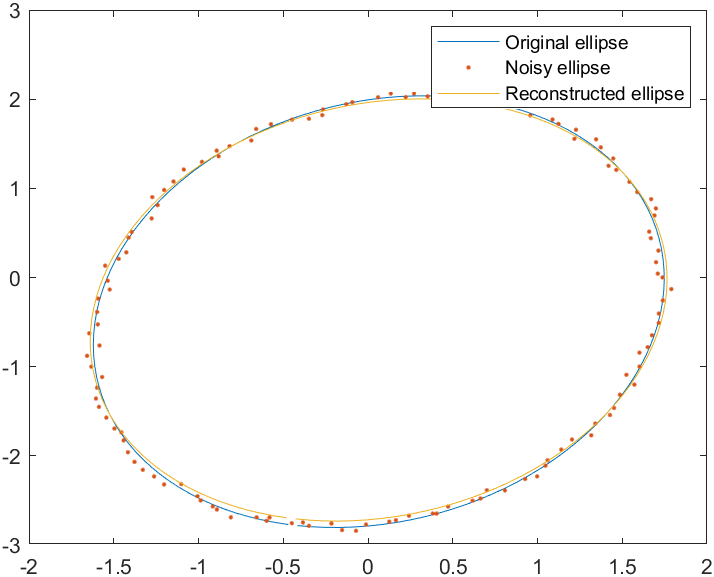
\includegraphics[width=0.5\linewidth]{Doc/Graphics/Part3/ReconstructedAsteroidTrajectory.png}
    \caption{Reconstructed asteroid trajectory}
    \label{fig:ReconstructedAsteroidTrajectory}
\end{figure}


\subsection{Shape-Based Approaches}

\textbf{Question 3:} Recall basic principle of shape detection in Computer Vision.

Now, let us consider one planet to be detected and characterised (Fig. 1) in 3 different configurations.

\textbf{Question 4:} Detect \& Characterise (position, size) the 1st planet in Conf. 1.

\textbf{Question 5:} What’s happen with Conf. 2 and Conf. 3?








\subsection{Contour-Based Approaches}

\textbf{Question 6:} Extract the planet (Conf. 1) using N points and next a Pseudo-Inverse Approach. What’s happen in other configurations?

\textbf{Question 7:} Extract the planet (Conf. 1) using N points and next a Pseudo-Inverse Approach. What’s happen in other configurations?

\textbf{Question 8:} Extract the planet (Conf. 1) using an Optimisation algorithm. What’s happen in other configurations?

\textbf{Question 9:} Explain the RANSAC Algorithm. Use it in Conf. 2 and Conf. 3.

\textbf{Question 10:} Compare with the circular Hough Transform.